\section{Validation of results}
\label{sec:validation}

\begin{itemize}
    \item[-] \textbf{Use publicly available tools to draw the ISS ground-track at the same epoch and compare it with your results.}
\end{itemize}

Using the ISSTracker tool we can plot a groundtrack of the ISS for the same timeperiod as in Section \ref{sec:ground_track}. 
For this, we first extract the epoch from the telemetry data and arrive at: $2024-10-07 \quad 12:48:15 \quad UTC$.
We can now input this to the ISSTracker (exchanging UTC for $+0000$) and see the correct plot in Figure Section \ref{fig:ISS_validation} below.

From the figure, especially the starting and ending points of the groundtrack, we see that our computed groundtrack matches this fairly well.
Additionally, the orbital period which arrived at in \ref{sec:TLE} of $5576.436740221023 \, s$ or $92.94061233701704 \, min$ matches the orbital period value found online of about $92,9 \, min$ \cite{ISS_tracking_orbitalperiod}.

As such, we can conclude that our method for computing and plotting the groundtrack in Section \ref{sec:TLE} is sound.

\begin{figure}[H]
    \centering
    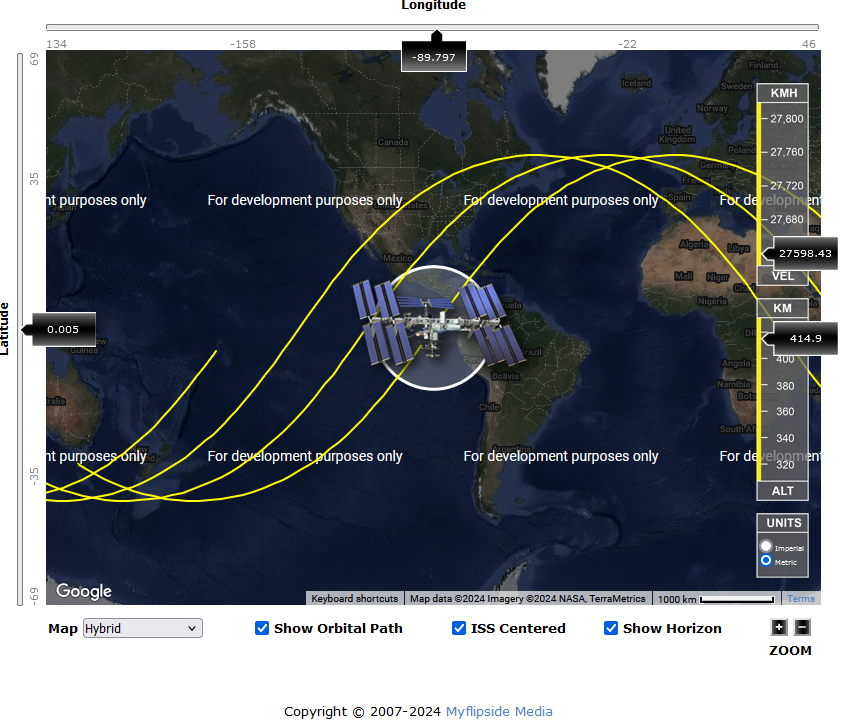
\includegraphics[width=0.8\linewidth]{Graphics/ISS_validation.png}
    \caption{Groundtrack of the ISS drawn at our epoch 2024-10-07 12:48:15+0000 (UTC) using online tool. \cite{ISStracker}}
    \label{fig:ISS_validation}
\end{figure}


